\documentclass[letterpaper, 10 pt, conference]{ieeeconf} 
\IEEEoverridecommandlockouts 
\overrideIEEEmargins                                      % Needed to meet printer requirements.
\usepackage{natbib}
\usepackage{graphicx}
\usepackage[ruled]{algorithm2e}

\title{\LARGE \bf
Interpreting Multimodal Referring Expressions in Real Time}
\author{Miles Eldon$^{1}$ and Stefanie Tellex$^{1}$
\thanks{$^{1}$Computer Science Department, Brown University}
}

\usepackage{amsfonts, amssymb, amsmath}
\usepackage[usenames,dvipsnames]{color}
\newcommand{\stnote}[1]{\textcolor{Blue}{\textbf{ST: #1}}}
\newcommand{\menote}[1]{\textcolor{Red}{\textbf{ME: #1}}}

\begin{document}

\maketitle
\thispagestyle{empty}
\pagestyle{empty}

\begin{abstract}
Robots that collaborate with humans must be able to identify objects
used for shared tasks, for example tools such as a knife for
assistance at cooking, or parts such as a screw on a factory floor.
Existing work has addressed this problem in single modalities, such as
natural language or gesture, but a gap remains in creating real-time
multimodal systems that simultaneously fuse information from language
and gesture in a principled mathematical framework.  We define a
multimodal Bayes' filter for interpreting referring expressions to
object using language and gesture in real time.  We collected a new
RGB-D and audio dataset of people referring to objects in a tabletop
setting and demonstrate that our approach successfully integrates
information from language and gesture in real time to quickly and
accurately identify objects continuously.
\end{abstract}

\section{INTRODUCTION}

In order for humans and robots to collaborate in complex tasks, robots
must be able to understand people's references to objects in the
external world.  To refer to objects, people use a combination of
language, hand gestures, and body language such as eye gaze.  These
signals are provided continuously to the robot over time, and can
change rapidly as a person responds to their environment.  For
example, Figure~\ref{fig:example} shows a robot handing a tool to a
human collaborator for a manufacturing task.  For the robot to infer
the correct tool to deliver, it must interpert a person's language and
gesture over time.

Most existing approaches for interpreting language and gesture rely on
unimodal models that do not integrate the two information sources,
even though people fluidly use language and gesture together.
Approaches that fuse information from language and
gesture~\citep{matuszek14} do not take into account that information
appears to the system over a period of time.  If a robot could exploit
this temporal information, it can respond in real time to a person's
input and indicate when it has understood; this backchannel feedback
could enable a person to respond and provide additional clarifying
input when the robot fails to understand.

To support these types of interactions, we propose a Bayes' filtering
approach for interpreting multimodal information from language and
gesture~\citep{thrun08}.  Our framework relies on a factored
observation probability that fuses information from language, hand
gestures, and head gestures in real time to continously estimate the
object a person is referring to in the real world.  We demonstrate our
model in simulation, as well as providing quantitative results on a
real-world RGB-D corpus of people referring to objects in the
environment.  These results demonstrate that our approach quickly and
accurately fuses multimodal information in real time to continously
estimate the object a person is referring to.

\begin{figure}
\centering
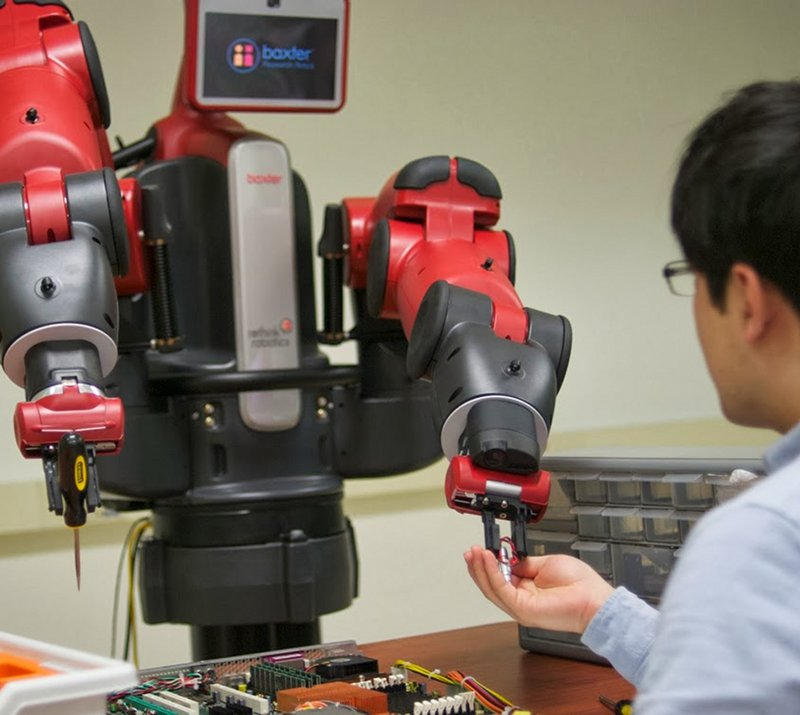
\includegraphics[width=1\linewidth]{figures/baxter_scene_cropped.jpg}
\caption{Robots that collaborate with people need to understand their
  references to objects in the environment.  For example, if a person
  asks for a tool using language and gesture, the robot needs to
  interpret the person's reference in order to pick up the correct
  tool.\label{fig:example}}
\end{figure}

\section{RELATED WORK}

Our approach is related to \citet{holladay14} but focuses on
interpreting a person's gestures rather than enabling a robot to
generate pointing gestures.  A large body of work focuses on language
understanding for robots~\citep{macmahon06, dzifcak09, kollar10,
  matuszek12}.  \citet{guadarrama14} presents a framework for
interperting open-domain references to objects but focuses on
interperting language rather than language combined with gesture.

Many existing approaches for interpreting gesture rely on fixed
vocabularies of gesture, such as ``stop'' or
``follow''~\citep{waldherr00, marge11} without a princepled way for
fusing information from language and gesture.  Our work unifies
language and gesture interpretation into a single mathematical
framework, and focuses on parameterized gestures such as pointing.


\citet{matuszek14} presented a multimodal framework for interpreting
unscripted references to tabletop objects using language and gesture.
Our approach similarly focuses on tabletop objects but uses language,
gesture, and head pose, and integrates these disparate data sources
continuously over time using a Bayes' filtering framework.  This
approach enables the robot to continuously process new information and
produce an estimate that converges over time to the correct object as
new information is observed from the person.  

\section{TECHNICAL APPROACH}

Our aim is to estimate a distribution over the object that a person is
referring to given language and gesture inputs.  We frame the problem
as a Bayes' filter~\citep{thrun08}, where the hidden state,
$\mathcal{X}$, is the set of $m$ objects in the scene that the person
is currently referencing. The robot observes the person's actions and
speech, $\mathcal{Z}$, and at each time step estimates a distribution
over $\mathcal{X}$:
\begin{align}
  p(x_t | z_0 \dots z_{0:t})
\end{align}


To estimate this distribution, we take a Bayes' filtering approach and
alternate performing a time update and a measurement update.  The time
update updates the belief that the user is referring to a specific
subset of objects given previous information:
\begin{align}
p(x_t | z_{0:t-1}) = \int p(x_t|x_{t-1})\times p(x_{t-1} | \mathcal{Z}_{0:t-1}) \text{d}x_{t-1}
\end{align}

The measurement update combines the previous belief with the newest observation to update each belief state: 
\begin{align}
p(x_t | \mathcal{Z}_{0:t}) = \frac{p(z_t | x_t) \times p(x_t | z_{0:t-1})}{p(z_t | z_{0:t-1})} \\\propto p(z_t | x_t) \times p(x_t | z_{0:t-1})
\end{align}

Algorithm~\ref{alg:algorithm} shows pseudocode for our approach.


\subsection{Prediction Model}

\stnote{Miles, can you check if this math is right?}

We assume that a person is likely to continue referring to the same
object, but at each timestep has a small probability, $c$, of
transitioning to a different object: 

\begin{align}
p(x_t | x_{t-1}) = \left\{  \begin{array}{ll}
1-c &\mbox{if } x_t = x_{t-1}\\
c &\mbox{otherwise}
\end{array}\right.
\end{align}

In our experiments, $c$ has a value of XXX.


\subsection{Observation Model}

We assume access to an observation model of the form:
\begin{align}
p(z_t | x_t)
\end{align}

Observations consist of a tuple consisting of a person's actions,
$\langle l, r, h, s\rangle $ where:
\begin{itemize}
	\item $l$ represents the observed origin ($l_o$) and vector ($l_v$) for the left arm.
	\item $r$ represents the observed origin  ($r_o$) and vector ($r_v$)  for the right arm .
	\item $h$ represents the observed origin  ($h_o$) and vector ($h_v$)  for head.
	\item $s$ represents the observed speech from the user, consisting of a list of words.
	\end{itemize}

Formally, we have:
\begin{align}
p(z_t | x_t) &= p(l, r, h, s | x_t)\\
\intertext{We factor assuming that each modality is independent of the others given the state (the true object that the person is referencing):}
&= p(l | x_t) \times p(r | x_t) \times p(h | x_t) \times p(s | x_t)
\end{align}

\noindent The following sections describe how we model each type of
input from the person.

\noindent{\bf Gesture.}  We model pointing gestures as a vector through three
dimensional space. We calculate the angle between the gesture vector
and the vector from the gesture origin to the mean of each cluster,
and then use the PDF of a Gaussian with trained variance to determine
the weight that should be assigned to that object. Let $\Phi(<origin>,
<point>, <point>)$ give the angle between the two points with the
given origin.
%We calculate the probability of a gesture by examining every three dimensional particle (denoted as $q$) in an object and calculating the angle (function $\Phi$) between the vector formed by the gesture and the vector formed with that particle. We then use a Gaussian distribution with a variance ($\sigma$) found during training to calculate the probability of seeing that angle difference. We then take the product of each of these points and normalize it so that small objects with few particles don't always dominate the probability distribution. The probability of each gesture given the state is as follows:
\begin{align}
p(l | x_t) \propto \mathcal{N}(\mu_l=0, \sigma_l,\Phi(l_o, l_v, x_t))\\
p(r | x_t) \propto \mathcal{N}(\mu_r=0, \sigma_r,\Phi(r_o, r_v, x_t))
%p(l|x_t) =[\displaystyle \prod_{q \in x_t} \mathcal{N}(\mu_l=0, \sigma_l, \Phi(l_o,l_v, q))]^{(\frac{\sum_{x'\in\mathcal{X}} len(x'_q)}{len(x_q)})}\\
%p(r|x_t) = [\displaystyle \prod_{q \in x_t} \mathcal{N}(\mu_r=0, \sigma_r, \Phi(r_o,r_v, q))]^{(\frac{\sum_{x'\in\mathcal{X}} len(x'_q)}{len(x_q)})}
\end{align}

\noindent{\bf Head Pose.}
Head pose is modeled in the same manner as arm gestures.
\begin{align}
p(h | x_t) \propto \mathcal{N}(\mu_h=0, \sigma_h,\Phi(h_o, h_v, x_t))
%p(h|x_t) = [\displaystyle \prod_{q \in x_t} \mathcal{N}(\mu_h=0, \sigma_h, \Phi(h_o,h_v, q))]^{(\frac{\sum_{x'\in\mathcal{X}} len(x'_q)}{len(x_q)})}
\end{align}


%\menote{More concise way to show this? They are all the same besides
%variance. I guess we could just do $\prod_{g\in\{h,l,r\}}$}
% stefie10: I think it's fine as is.  It's okay to duplicate it.  I
% think it's easier to understand that way.


\noindent{\bf Speech.}
We model speech with a simple bag of words model. We take the words in a given speech input and count how many words in this text match descriptors (denoted  $x_d$) of specific objects.
\begin{align}
p(s |x_t) = \displaystyle \prod_{w \in s} p(w | x_t)
\end{align}

\subsection{Training Model Parameters}

We train model parameters by fitting each factor to a ground-truth
distribution.

\begin{algorithm}
    \DontPrintSemicolon
    \KwIn{$bel(x_{t-1}), u_t, z_t$}
    \BlankLine
    \KwOut{$bel(x_t)$}
    \BlankLine
    \For{ $x_t$} {
      $\bar{bel}(x_t) = $
      \BlankLine
      $bel(x_t) = $

    }
    \BlankLine
      \stnote{Miles -- can you fill in the algorithm?  We shouldn't just reproduce a simple Bayes' filter; it should get into what specific things we had to do to make it work with multimodal input.}
\caption{Interactive Bayes Filtering Algorithm} 
\label{alg:algorithm}
\end{algorithm}



\section{EVALUATION}

We evaluate our model in simulation, comparing the full model to
versions without multimodal information.  Additionally we assessed its
performance on an RGB-D audio and video corpus of people referring to
objects.  Finally we created an end-to-end robotic demonstration,
demonstrated in the video attachement to our paper, and available
online\footnote{video reference}. 

\subsection{Simulation Results}

\subsection{Real-world Corpus-Based Results}

\begin{figure}
\parbox{1\linewidth}{~\\~\\~\\~\\}
\caption{Scene from our dataset.\label{fig:corpus_scene}}
\end{figure}

Our real-world experiments measured our algorithm's performance when a
person referred to an object visually and with gesture.  The person
was seated roughly five feet from a table which had several objects,
as shown in Figure~\ref{fig:corpus_scene}.  We instructed them to
refer to the object as if they were talking to another person, using
language and gesture.  We indicted the object to refer to using a
laser pointer, and we periodically shifted to a different object on a
predetermined schedule.  They wore a microphone to pick up
high-quality audio, and we tracked their body pose using the NITE
tracker~\citep{openni}.  We used the Google Voice Recognition package
to recognize speech.  We used two Kinects: one pointed outward at the
person, and one pointed down to recognize objects on the table.

\begin{table}
\begin{tabular}{cc}
Language only &  XX\\
Gesture only  &  XX\\
Head only     &  XX\\
Multimodal    &  XX\\
\end{tabular}
\caption{Real-world Results}
\end{table}

\subsection{Robotic Demonstration}

Because our approach enables a robot to quickly and constantly monitor
a person's references to an object, a robot can respond to these
estimates in real time.  We demonstrate this behavior by enabling
Baxter to demonstrate its certainty about what object is being
referenced, this eliciting more feedback from the person.  When the
robot is very unsure, its arm moves back and forth between the
candidate objects.  When it is sure, then it moves with more
precision.  The video shows this behavior, as a person provides more
information about what object is being referred to by the person.

\section{CONCLUSION}

We have demonstrated a Bayes' filtering approach to interperting a
person's multimodal language and gesture references to objects
continoulsly in real time.  Our approach enables a robot to understand
a person's references to objects in the real world.

In the future we plan to expand our language model to incorporate
models of compositional semantics and lower-level visual features so
that the robot is not limited to prespecified object models.


\bibliographystyle{abbrvnat}
\bibliography{main}



\end{document}
